\documentclass{article}
\usepackage[german]{babel}
\usepackage{float}
\usepackage{fourier}
\usepackage[utf8]{inputenc}
\usepackage[T1]{fontenc}
\usepackage{amsfonts,amsthm, amsmath}
\usepackage{listings}
% The following is needed in order to make the code compatible
% with both latex/dvips and pdflatex.
\ifx\pdftexversion\undefined
\usepackage[dvips]{graphicx}
\else
\usepackage[pdftex]{graphicx}
\DeclareGraphicsRule{*}{mps}{*}{}
\fi

\setlength\parindent{0pt}
\lstset{language=Erlang}

\begin{document}

\textbf{Team:} TEAM 01, Falco Winkler (FW), Daniel Schruhl (DS)\\
\\
\textbf{Aufgabenteilung:}
\begin{itemize}
    \item DLQ (DS)
    \item CMEM (DS)
	\item HBQ (FW)
\end{itemize}

\textbf{Quellenangaben:}\\
\\
\textbf{Bearbeitungszeitraum:}
\begin{itemize}
	\item 26.03.2017 (FW,DS)
	\item 03.04.2017 (DS)
	\item 04.04.2017 (DS)
\end{itemize}

\textbf{Aktueller Stand:}
\begin{itemize}
	\item DLQ fertig und getestet
	\item CMEM fertig und getestet
	\item HBQ angefangen
	\item Server
	\item Client
\end{itemize}

\textbf{Änderung des Entwurfs:}
\begin{itemize}
    \item Formatierung angepasst
	\item Komponentendiagramm erweitert
	\item Detailbeschreibungen für jedes Modul und Pakete
\end{itemize}

\newpage
\tableofcontents 
\newpage

\section{Einführung und Ziele}
Es soll eine Message of the Day Anwendung erstellt werden. Dabei werden von verschiedenen Clients an einen Server verschiedene Nachrichten des Tages gesendet. Die Clients rufen vom Server alle Nachrichten ab, so dass jeder Client alle Nachrichten in einer festen Reihenfolge hat.

\subsection{Randbedingungen}
Es soll eine Client/Server-Architektur implementiert werden.
Der Server verwaltet dabei die ihm von den Clients gesendeten Nachrichten. Das beinhaltet eine feste Numerierung der Nachrichten.

Die Clients rufen dabei in bestimmten Abständen die Nachrichten ab. Falls ein Client dem Server schon bekannt ist, bekommt der nur die ihm noch unbekannten (neuen) Nachrichten.

Der Server muss sich also die Clients merken. Es soll mit einer Holdbackqueue und einer Deliveryqueue gearbeitet werden, um die korrekte Auslieferung in einer bestimmten Reihenfolge der Nachrichten zu garantieren.

\subsection{Kontextbegrenzung}
Das System soll in Erlang umgesetzt werden. Es muss auf Computern mit Linux Betriebssystem lauffähig sein.

\newpage

\section{Gesamtsystem}

\subsection{Bausteinsicht}
Das Softwareprodukt besteht aus mehreren Modulen und Paketen (Abbildung \ref{fig:component-diagram}). Diese Pakete setzen sich zusammen aus dem Client-Paket und dem Server-Paket.

\begin{figure}[H]
    \centering
    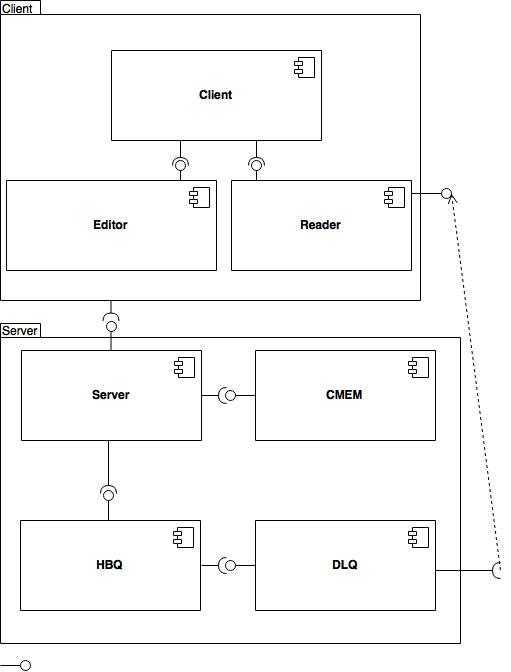
\includegraphics[width=0.5\textwidth]{component-diagram.png}
    \caption[seq-dia]{Komponentendiagramm der Message Of The Day App}
    \label{fig:component-diagram}
\end{figure}

Das Server Paket beinhaltet das Server-Modul und alle vom Server-Modul verwendeten Datenstrukturen.\\
Das Server-Modul ist für alle Funktionalitäten des Servers zuständig. Dazu gehört das Nummerieren und Verwalten der Nachrichten und die Verwaltung der Clients.\\
Das Server-Modul benutzt daher per Schnittstelle das HBQ-Modul und das CMEM-Modul. Das Server-Modul stellt eine Schnittstelle für die Clients bereit.\\
\\
Das CMEM-Modul ist für die Speicherung der Clients und ihrer aktuellen zu erwartenden Nachrichten Nummer zuständig. Das CMEM-Modul soll als lokale ADT realisiert werden. Diese wird nur vom Server angesprochen.\\
\\
Das HBQ-Modul ist für die Holdbackqueue zuständig und regelt die Sortierung der einkommenden Nachrichten in die Deliveryqueue und der damit verbundenen Fehlerbehandlung. Dabei ist das HBQ-Modul als entfernte ADT realisiert. Diese wird nur von dem Server-Modul verwendet.\\
\\
Das DLQ-Modul realsiert die Deliveryqueue, die für die Auslieferung der Nachrichten in Reihenfolge an die Clients zuständig ist. Die Schnittstelle des DLQ-Moduls wird nur vom HBQ-Modul konsumiert.\\
\\
Das Client-Paket beinhaltet die Client-Module. Diese sind zum einen der Lese Client (Reader-Modul) und der Redakteur Client (Editor-Modul). Beide Clients sind als ein Prozess implementiert und verwenden die vom Server bereitgestellte Schnittstelle. Der Redakteur Client ist für das Schicken von Nachrichten zuständig und der Lese Client für das Lesen von Nachrichten.

\subsection{Laufzeitsicht}
\begin{figure}[H]
\centering
\includegraphics[width=\textwidth]{sequence-diagram.png}
\caption[seq-dia]{Sequenzdiagramm bei fehlerfreiem Nachrichtenaustausch}
\label{fig:sequence-diagram}
\end{figure}

\newpage

\section{Subsysteme und Komponenten}

\subsection{Server}
\subsubsection{Aufgabe und Verantwortung}
Der Server hat die Aufgaben  
\begin{enumerate}
	\item{Sich anfragende Clients mit ProzessID und Zeitstempel zu merken}
    \item{Clients die ihnen zugehörigen Nachrichten zurückzugeben}
\end{enumerate}
Für die erste Aufgabe wird das Modul CMEM verwendet. 
Zum Senden an die Clients leitet der Server die Nachrichten zunächst an die HBQ weiter. 
Erscheint eine Anfrage vom Client, erfolgt über die HBQ der Aufruf an die DLQ, die Nachricht zu übermitteln.

\subsubsection{Entwurfsentscheidungen}
Der Server bearbeitet Anfragen per message passing. Die NNr ist ein Zählerwert, der nach jedem Herausgeben an einen Client inkrementiert wird.

\subsubsection{Außensicht}
Es werden Schnittstellen zur Abfage der aktuellen NNr, zum Holen \& Speichern von Nachrichten bereitgestellt. Nach einer bestimmten, aber nach Außen unbekannten Zeit werden auch bereits abgeholte Nachrichten ausgeliefert.

\subsubsection{Innensicht}
Anfragen werden in einer Endlosschleife abgefragt und nur an die jeweiligen Komponenten weitergeleitet. Fehlerbehandlung erfolgt in den jeweiligen Komponenten. Bei jeder Anfrage erfolgt die Abfrage \& Aktualisierung der CMEM, um sich den anfragenden Client zu merken und Anfragen an die HBQ korrekt zu stellen.
			
\subsubsection{Konfigurationsparameter}
\begin{enumerate}
    \item{Latenzzeit bestimmt die maximale Zeit die der Server ungenutzt läuft.}
    \item{Lebenszeit des Clients bestimmt die Zeit, für die sich der Server einen Client merkt.}
    \item{Name definiert den Namen der Server - Node}
    \item{HBQ - Name \& Node definieren die Verknüpfung zur HBQ - Node}
\end{enumerate}

\subsubsection{Benutzungsschnittstelle}
Der Server wird nur durch seine Schnitstellen vom Client verwendet.
\newpage

\subsection{CMEM-Modul}
\subsubsection{Aufgabe und Verantwortung}
Dieses Modul hat die Aufgabe sich anfragende Clients, ihre letzte bekommene Nachrichtennummer und den letzten Zeitpunkt ihrer Anfrage zu merken.
Clients, die sich seit einiger Zeit (Konfigurationsparameter) nicht gemeldet haben, sollen aus dem CMEM-Modul gelöscht werden können.

Die gespeicherten Daten sollen über die Schnittstelle des Moduls vom Server aus abrufbar sein.

\subsubsection{Schnittstelle}
\begin{lstlisting}[language=erlang]
/* Initialisieren des CMEM */
initCMEM(RemTime,Datei): Integer X Atom -> CMem

/* Speichern/Aktualisieren eines Clients in dem CMEM */
updateClient(CMEM,ClientID,NNr,Datei): Cmem X PID X Integer X Atom -> CMem

/* Abfrage welche Nachrichtennummer der Client als naechstes erhalten darf */
getClientNNr(CMEM,ClientID) : Cmem X PID -> Integer
\end{lstlisting}

\textbf{initCMEM(RemTime,Datei)}: initialisiert den CMEM. RemTime gibt dabei die Zeit an, nach der die Clients vergessen werden Bei Erfolg wird ein leeres CMEM zurück geliefert. Datei kann für ein logging genutzt werden.\\

\textbf{updateClient(CMEM,ClientID,NNr,Datei)}: speichert bzw. aktualisiert im CMEM den Client ClientID und die an ihn gesendete Nachrichtenummer NNr. Datei kann für ein logging genutzt werden.\\

\textbf{getClientNNr(CMEM,ClientID)}: gibt die als nächstes vom Client erwartete Nachrichtennummer des Clients ClientID aus CMEM zurück. Ist der Client unbekannt wird 1 zurück gegeben.\\

\subsubsection{Entwurfsentscheidungen}
Die CMEM wird mit Hilfe einer Liste realisiert. An erster Stelle der CMEM Liste steht die Liste der Clients. Die Elemente der Client Liste sind Tupel, die aus der Client Prozess ID, der zuletzt erhaltenen NNr und einem Timestamp der letzten Aktion in Millisekunden bestehen.

An zweiter Stelle der CMEM Liste steht die maximale Zeit, für die ein Client gemerkt wird in Millisekunden.

\begin{lstlisting}[language=erlang]
/* Client Tupel Format */
Client := {ClientPID,NNr,ClientTS}:
    {PID X Integer X Integer}

/* CMEM Format */
/* ClientList ist Liste bestehend aus Clients */
/* RemTime ist Zeit in Millisekunden fuer die Clients gemerkt werden */
CMEM := [ClientList, RemTime]: [List X Integer]
\end{lstlisting}

Falls beim Aktualisieren eines Clients der Client noch nicht im CMEM steht, wird er hinzugefügt.
Ansonsten wird er einfach mit den angegebenen Parametern in der CMEM Client Liste aktualisiert.\\

Wenn die nächste Nachrichtennummer für einen Client abgerufen wird (\texttt{getClientNNr}), wird ein Check gemacht, ob der Client bekannt ist.
Ein Client ist bekannt, wenn er in der CMEM Liste steht und wenn die Summe seines Timestamps mit der RemTime größer gleich der aktuellen Zeit (als Timestamp) ist.\\

Für bekannte Clients wird die resultierende nächste Nachrichtennummer inkrementiert. Für unbekannte Clients wird 1 als nächste Nachrichtennummer zurück gegeben.

\subsubsection{Konfigurationsparameter}
\begin{enumerate}
    \item{Zeit nach der die Clients vergessen werden in Millisekunden (RemTime)}
\end{enumerate}

\newpage
			
\subsection{Komponente HBQ}
\subsubsection{Aufgabe und Verantwortung der HBQ}
Von Redakteur-Clients gesendete Nachrichten werden hier zwischengespeichert. Gibt es keine Lücke in der fortlaufenden Nummerierung der Nachrichten, werden Sie an die DLQ weitergeleitet. Bei einer Überfüllung der HBQ (2/3 der Maximalen Kapazität der DLQ) wird die älteste Lücke in den Nachrichten mit einer künstlichen Nachricht geschlossen, und es werden erneut alle Lückenlosen Nachrichten an die DLQ weitergeleitet. Die HBQ stellt nur ein Interface für den Server bereit.

\subsubsection{Entwurfsentscheidungen}
Es wird die Aktuelle NNr gespeichert.
Jede Nachricht, die der aktuellen erwarteten NNr entspricht, wird direkt weitergeleitet.
Wenn noch auf alte Nachrichten gewartet wird, wird die nachricht in die HBQ eingefügt.
Wenn die Nachrichtennummer größer als der erwarteten Nachrichtennummer ist,
müssen alle bereits empfangenennachrichten ab der erwarteten Nachrichtennummer durchgegangen werden.
Die Nachrichten, die aufeinanderfolgende Sequenznummern haben werden an die
DLQ ausgeliefert.
				
if currentNNr == NNr
	currentNNr +=1
	pushToDLQ(NNr)
else
	insert(NNr)
	currentNNr = pushAllConsecutiveFrom(currentNNr) 
				
\subsubsection{Außensicht}

\subsubsection{Innensicht}

\subsubsection{Konfigurationsparameter}
\begin{itemize}
	\item Die Maximalgröße der DLQ wird verwendet um die HBQ bei kritischer Überfüllung zu leeren.
\end{itemize}
\newpage

\subsection{DLQ-Modul}
\subsubsection{Aufgabe und Verantwortung}
Die Deliveryqueue hat die Aufgabe Nachrichten an Clients zuzustellen und stellt eine Datenstruktur dar, die eine maximale Menge (Kapazität) an Nachrichten hält. Sie verhält sich dabei wie von einer Warteschlange zu erwarten beim Einfügen und Herausholen von Nachrichten (FIFO). Nur das HBQ-Modul darf auf das DLQ-Modul zugreifen. Das DLQ-Modul sendet über eine Schnittstelle der Clients die Nachrichten an die Clients.

\subsubsection{Schnittstelle}
\begin{lstlisting}[language=erlang]
/* Initialisieren der DLQ */
initDLQ(Size,Datei): Integer X Atom -> DQueue

/* Abfrage welche Nachrichtennummer in der DLQ gespeichert werden kann */
expectedNr(Queue) : DQueue -> Integer

/* Speichern einer Nachricht in der DLQ */
push2DLQ([NNr,Msg,TSclientout,TShbqin],Queue,Datei) :
    MSG_list X DQueue X Atom -> DQueue

/* Ausliefern einer Nachricht an einen Leser-Client */
deliverMSG(MSGNr,ClientPID,Queue,Datei):
    Integer X PID X DQueue X Atom -> Integer
\end{lstlisting}

\textbf{initDLQ(Size,Datei)}: initialisiert die DLQ mit Kapazität Size. Bei Erfolg wird eine leere DLQ zurück geliefert. Datei kann für ein logging genutzt werden.\\

\textbf{expectedNr(Queue)}: liefert die Nachrichtennummer, die als nächstes in der DLQ gespeichert werden kann. Bei leerer DLQ ist dies 1.\\

\textbf{push2DLQ([NNr,Msg,TSclientout,TShbqin],Queue,Datei)}: speichert die Nachricht [NNr,Msg,TSclientout,TShbqin] in der DLQ Queue und fügt ihr einen Eingangszeitstempel an (einmal an die Nachricht Msg und als expliziten Zeitstempel TSdlqin mit erlang:now() an die Liste an. Bei Erfolg wird die modifizierte DLQ zurück geliefert. Datei kann für ein logging genutzt werden.\\

\textbf{deliverMSG(MSGNr,ClientPID,Queue,Datei)}: sendet die Nachricht MSGNr an den Leser-Client ClientPID. Dabei wird ein Ausgangszeitstempel TSdlqout mit erlang:now() an das Ende der Nachrichtenliste angefügt. Sollte die Nachrichtennummer nicht mehr vorhanden sein, wird die nächst größere in der DLQ vorhandene Nachricht gesendet. Bei Erfolg wird die tatsächlich gesendete Nachrichtennummer zurück geliefert. Datei kann für ein logging genutzt werden.\\

\subsubsection{Entwurfsentscheidungen}
Die Deliveryqueue wird als Liste realisiert. Das erste Element der Liste ist dabei eine Liste der Nachrichten und das zweite Element der Liste gibt die Kapazität der DLQ an.
\begin{lstlisting}[language=erlang]
/* Nachrichten Format */
/* minimal 3 Elemente, pro Station kommt eins hinzu; maximal 6 Elemente */
MSG_List := [NNr,Msg,TSclientout,TShbqin,TSdlqin]:
    [Integer X String X 3-Tupel X 3-Tupel X 3-Tupel]

/* DLQ Format */
/* Nachrichtenliste ist eine Liste aus MSG_List und hat */
/* maximal Kapazitaet Anzahl an Elementen */
DLQ := [Nachrichtenliste, Kapazitaet]: [List X Integer]
\end{lstlisting}

Neue Nachrichten werden am Anfang der Liste angefügt. Das vereinfacht die Nachfrage nach der nächsten zu speichernden Nachrichtennummer in der DLQ. Demnach werden Nachrichten am Ende der Liste entnommen. Wenn eine Nachricht in die DLQ eingetragen wird, wird ans Ende der Nachricht der aktuelle Zeitstempel zum Zeitpunkt des Einfügens hinzugefügt.

Nachrichten werden der DLQ entnommen, wenn die Größe der Liste gleich ihrer Kapazität ist und eine neue Nachricht hinzugefügt werden soll.\\

Beim senden einer Nachricht durch Angabe der Nachrichtennummer wird in der DLQ nach der Nachricht mit der Nachrichtennummer gesucht. Wenn diese gefunden wird, wird die Nachricht an den Client (mit der ClientPID) gesendet und die Nachrichtennummer zurück gegeben.

Falls die Nachricht nicht gefunden werden konnte, wird die nächste Nachricht mit der nächst größeren Nachrichtennummer an den Client gesendet. Diese wird mit einer Hilfsfunktion ermittelt (via reduce/foldl).

Beim senden einer Nachricht wird die Nachricht zusammen mit einem boolean Flag an den Client gesendet. Dieser boolean Flag signalisiert, ob noch weitere Nachrichten folgen.

Das wird mit einer weiteren Hilfsfunktion \texttt{remainingMessagesExist(MsgNr,DLQ)}) ermittelt.

Diese Hilfsfunktion holt sich den Kopf der DLQ Nachrichtenliste (aktuellste Nachricht mit höchster Nachrichtennummer) und vergleicht, ob diese Nachrichtennummer größer ist als die übergebene \texttt{MsgNr}.

\subsubsection{Konfigurationsparameter}
\begin{itemize}
    \item Kapazität der DLQ als ganze Zahl
\end{itemize}

\end{document}